\documentclass{article}
\usepackage[utf8]{inputenc}
\usepackage{hyperref}
\usepackage{amsmath}
\usepackage{amssymb}
\usepackage{geometry}
\usepackage{graphicx}
\usepackage{float}
\usepackage{fancyhdr}
\usepackage{listings}
\usepackage{float}

\pagestyle{fancy}
\fancyhf{}
\fancyhead[L]{Conception de Base de Données - TP1 Partie 2}
\fancyhead[R]{SANNA Thomas, L3STI}
\fancyfoot[C]{Page n°\thepage}
\fancyfoot[R]{Università di Corsica}

\title{Conception de Base de Données: \\ TP1 Partie 2 - Exercices}
\author{SANNA Thomas}
\date{\today}

\begin{document}

\begin{figure}
  \centering
  
\includegraphics[width=0.5\textwidth]{img/logoUniv.jpg}
  \label{fig:mysql-logo}
\end{figure}

\maketitle

\break\tableofcontents

\break\section{Question 1}

\subsection{Modèle Conceptuel de Données (MCD)}

\begin{figure}[H]
  \centering
  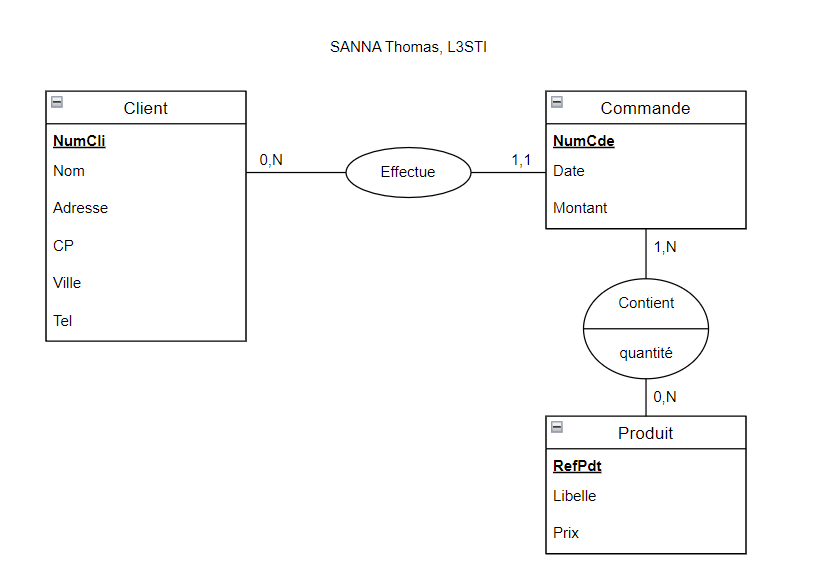
\includegraphics[width=1\textwidth]{graphs/mcd.png}
  \caption{Modèle Conceptuel de Données, en utilisant Draw.io.}
  \label{fig:MCD}
\end{figure}

\subsection{Couverture Minimale}

\begin{figure}[H]
  \centering
  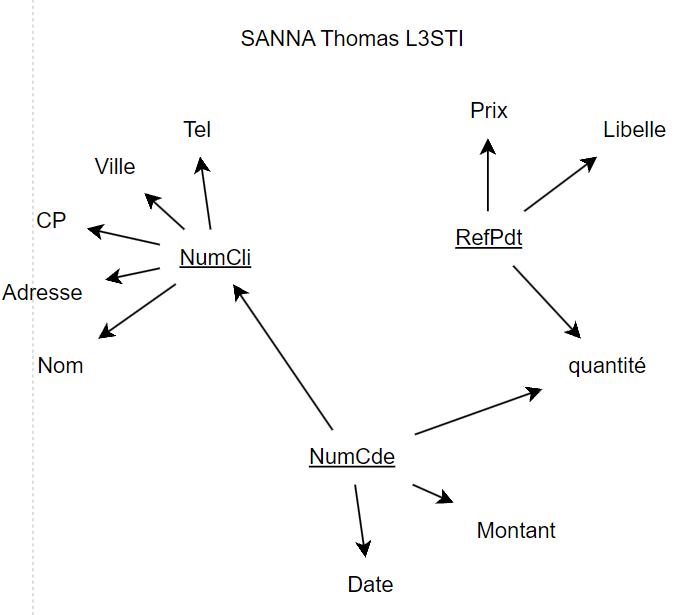
\includegraphics[width=0.8\textwidth]{graphs/couv-mini.png}
  \caption{Couverture Minimale, en utilisant Draw.io.}
  \label{fig:CM}
\end{figure}

\break\section{Question 2}

\subsection{Afficher tous les clients qui habitent Corte ou Omessa}

\subsubsection{Algèbre Relationnelle}

\begin{figure}[H]
  \centering
  
\includegraphics[width=0.7\textwidth]{alg/1.png}
  \label{fig:alg-rel}
\end{figure}

\begin{figure}[H]
  \centering
  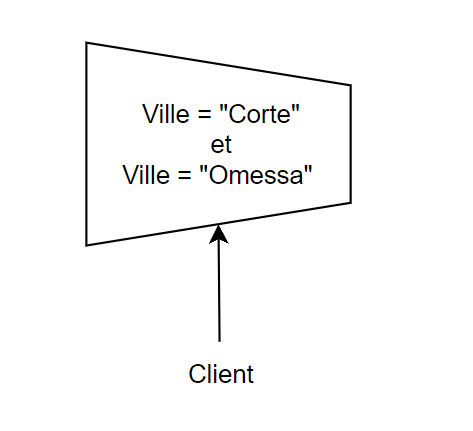
\includegraphics[width=0.5\textwidth]{algRel/1.png}
  \label{fig:alg-rel}
\end{figure}

\subsubsection{SQL}

\begin{lstlisting}[language=SQL]
  SELECT * 
  FROM Client 
  WHERE Ville = 'Corte' OR Ville = 'Omessa';  
\end{lstlisting}

\subsection{Afficher les noms et villes des clients}

\subsubsection{Algèbre Relationnelle}

\begin{figure}[H]
  \centering
  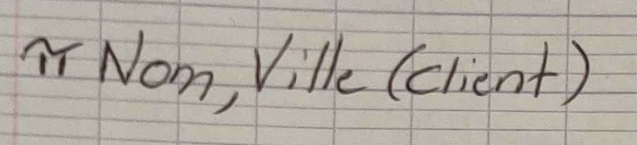
\includegraphics[width=0.5\textwidth]{alg/2.png}
  \label{fig:alg-rel}
\end{figure}

\begin{figure}[H]
  \centering
  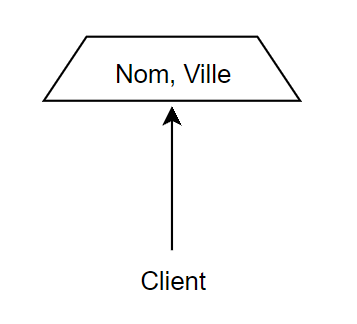
\includegraphics[width=0.5\textwidth]{algRel/2.png}
  \label{fig:alg-rel}
\end{figure}


\subsubsection{SQL}

\begin{lstlisting}[language=SQL]
  SELECT Nom, Ville 
  FROM Client;
\end{lstlisting}

\subsection{Afficher les noms et téléphones des Clients habitant Porto-Vecchio}

\subsubsection{Algèbre Relationnelle}

\begin{figure}[H]
  \centering
  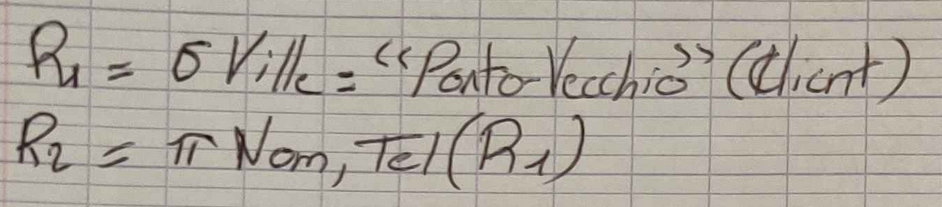
\includegraphics[width=0.7\textwidth]{alg/3.png}
  \label{fig:alg-rel}
\end{figure}

\begin{figure}[H]
  \centering
  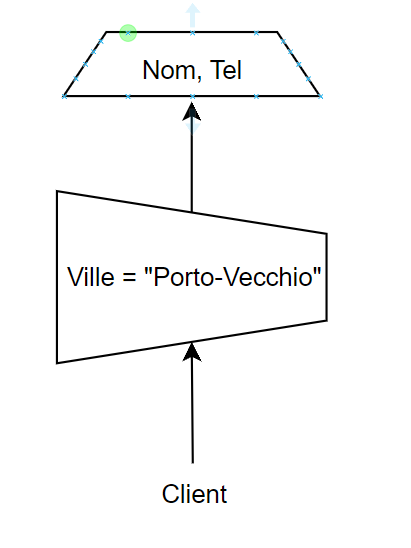
\includegraphics[width=0.5\textwidth]{algRel/3.png}
  \label{fig:alg-rel}
\end{figure}


\subsubsection{SQL}

\begin{lstlisting}[language=SQL]
  SELECT Nom, Tel 
  FROM Client 
  WHERE Ville = 'Porto-Vecchio';
\end{lstlisting}

\subsection{Afficher les noms de clients ayant passé une commande le 10/11/2020}

\subsubsection{Algèbre Relationnelle}

\begin{figure}[H]
  \centering
  
\includegraphics[width=0.7\textwidth]{alg/4.png}
  \label{fig:alg-rel}
\end{figure}

\begin{figure}[H]
  \centering
  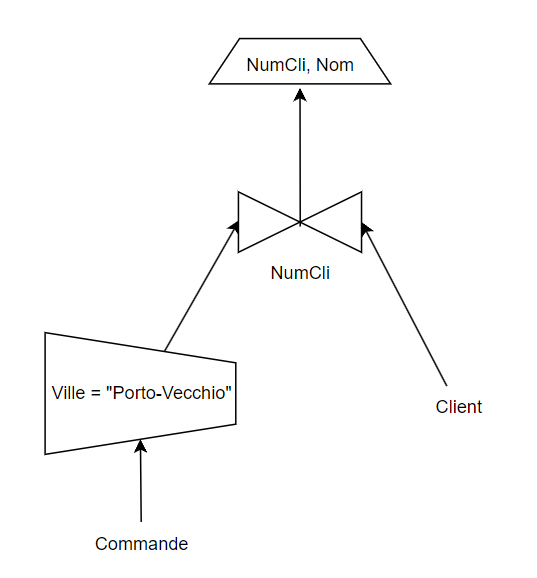
\includegraphics[width=0.5\textwidth]{algRel/4.png}
  \label{fig:alg-rel}
\end{figure}


NB : Pour les prochaines questions qui le demandent, j'ai aussi décidé de mettre NumCli en plus de Nom, pour plus de clarté et de précision.

\subsubsection{SQL}

\begin{lstlisting}[language=SQL]
  SELECT c.NumCli, c.Nom 
  FROM Client c
  JOIN Commande co ON c.NumCli = co.NumCli
  WHERE co.Date = '2020-11-10';
\end{lstlisting}

Version sans JOIN :

\begin{lstlisting}[language=SQL]
  SELECT c.NumCli, c.Nom 
  FROM Client c, Commande co 
  WHERE c.NumCli = co.NumCli 
    AND co.Date = '2020-11-10';
\end{lstlisting}

\subsection{Afficher les produits achetés par le client 102}

\subsubsection{Algèbre Relationnelle}

\begin{figure}[H]
  \centering
  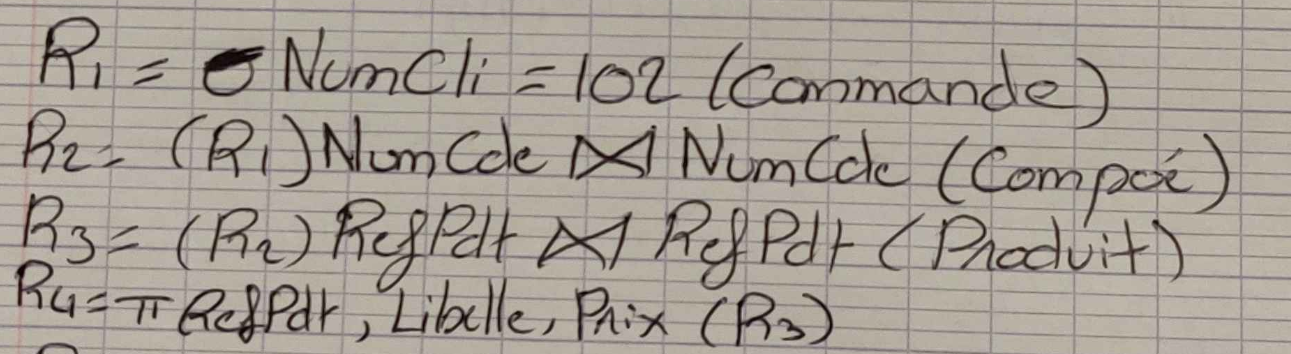
\includegraphics[width=0.7\textwidth]{alg/5.png}
  \label{fig:alg-rel}
\end{figure}

\begin{figure}[H]
  \centering
  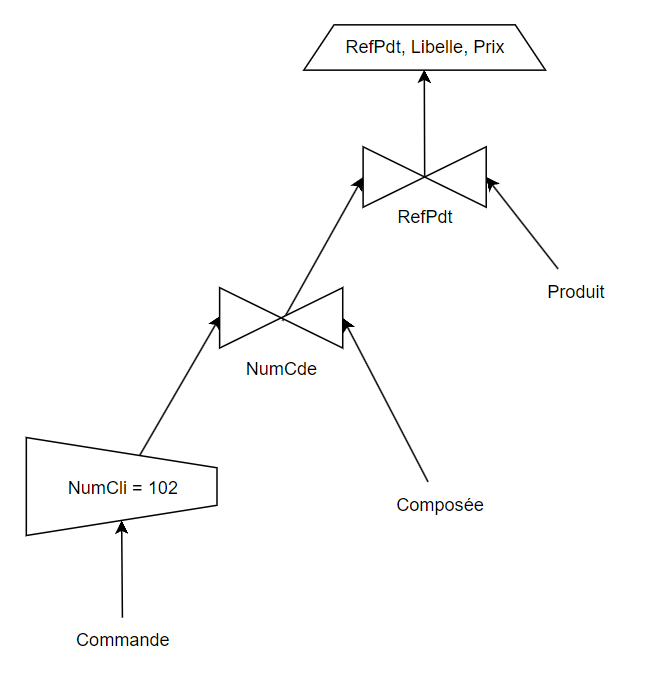
\includegraphics[width=0.5\textwidth]{algRel/5.png}
  \label{fig:alg-rel}
\end{figure}


\subsubsection{SQL}

\begin{lstlisting}[language=SQL]
  SELECT p.RefPdt p.Libelle 
  FROM Produit p
  JOIN Composee cp ON p.RefPdt = cp.RefPdt
  JOIN Commande c ON cp.NumCde = c.NumCde
  WHERE c.NumCli = 102;
\end{lstlisting}

Version sans JOIN :

\begin{lstlisting}[language=SQL]
  SELECT p.RefPdt p.Libelle 
  FROM Produit p, Composee cp, Commande c
  WHERE p.RefPdt = cp.RefPdt 
    AND cp.NumCde = c.NumCde 
    AND c.NumCli = 102;
\end{lstlisting}

\subsection{Afficher les produits achetés par le client "Delhom"}

\subsubsection{Algèbre Relationnelle}

\begin{figure}[H]
  \centering
  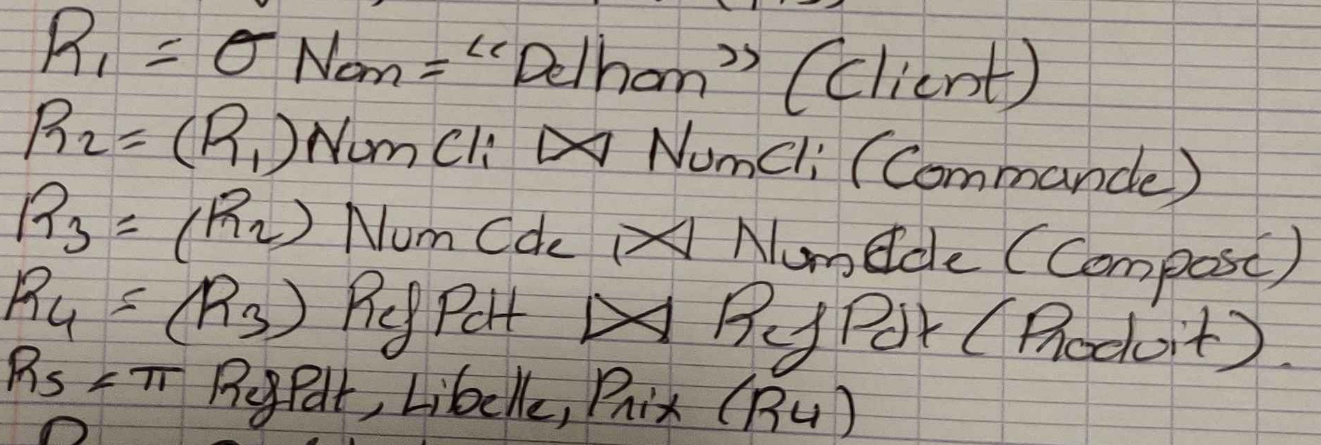
\includegraphics[width=0.7\textwidth]{alg/6.png}
  \label{fig:alg-rel}
\end{figure}

\begin{figure}[H]
  \centering
  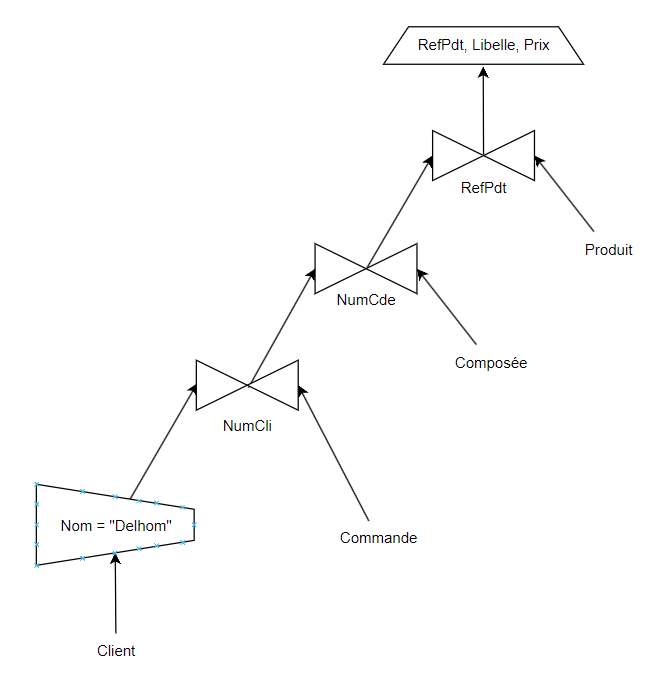
\includegraphics[width=0.5\textwidth]{algRel/6.png}
  \label{fig:alg-rel}
\end{figure}


\subsubsection{SQL}

\begin{lstlisting}[language=SQL]
  SELECT p.RefPdt, p.Libelle 
  FROM Produit p
  JOIN Composee cp ON p.RefPdt = cp.RefPdt
  JOIN Commande c ON cp.NumCde = c.NumCde
  JOIN Client cl ON c.NumCli = cl.NumCli
  WHERE cl.Nom = 'Delhom';
\end{lstlisting}

Version sans JOIN :

\begin{lstlisting}[language=SQL]
  SELECT p.RefPdt, p.Libelle 
  FROM Produit p, Composee cp, Commande c, Client cl
  WHERE p.RefPdt = cp.RefPdt 
    AND cp.NumCde = c.NumCde 
    AND c.NumCli = cl.NumCli 
    AND cl.Nom = 'Delhom';
\end{lstlisting}

\subsection{Noms des clients ayant acheté du Chocolat}

\subsubsection{Algèbre Relationnelle}

\begin{figure}[H]
  \centering
  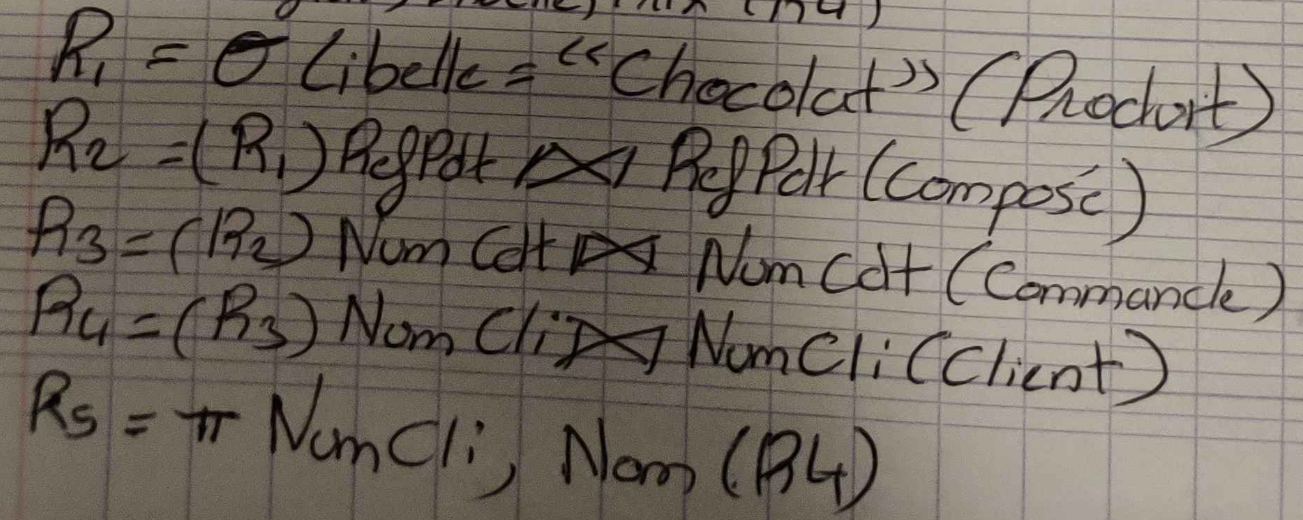
\includegraphics[width=0.7\textwidth]{alg/7.png}
  \label{fig:alg-rel}
\end{figure}

\begin{figure}[H]
  \centering
  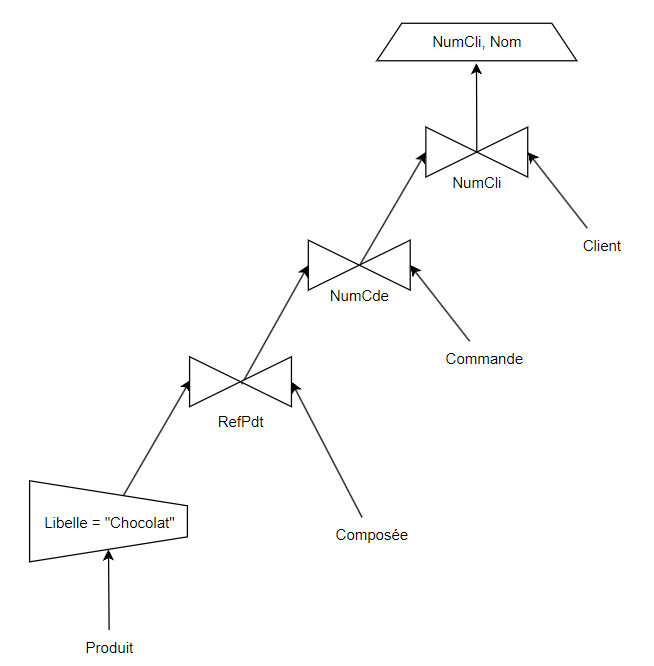
\includegraphics[width=0.5\textwidth]{algRel/7.png}
  \label{fig:alg-rel}
\end{figure}


\subsubsection{SQL}

\begin{lstlisting}[language=SQL]
  SELECT cl.NumCli, cl.Nom 
  FROM Client cl
  JOIN Commande c ON cl.NumCli = c.NumCli
  JOIN Composee cp ON c.NumCde = cp.NumCde
  JOIN Produit p ON cp.RefPdt = p.RefPdt
  WHERE p.Libelle = 'Chocolat';
\end{lstlisting}

Version sans JOIN :

\begin{lstlisting}[language=SQL]
  SELECT cl.NumCli, cl.Nom 
  FROM Client cl, Commande c, Composee cp, Produit p
  WHERE cl.NumCli = c.NumCli 
    AND c.NumCde = cp.NumCde 
    AND cp.RefPdt = p.RefPdt 
    AND p.Libelle = 'Chocolat';
\end{lstlisting}

\subsection{Noms des clients n’ayant jamais acheté de lait}

\subsubsection{Algèbre Relationnelle}

\begin{figure}[H]
  \centering
  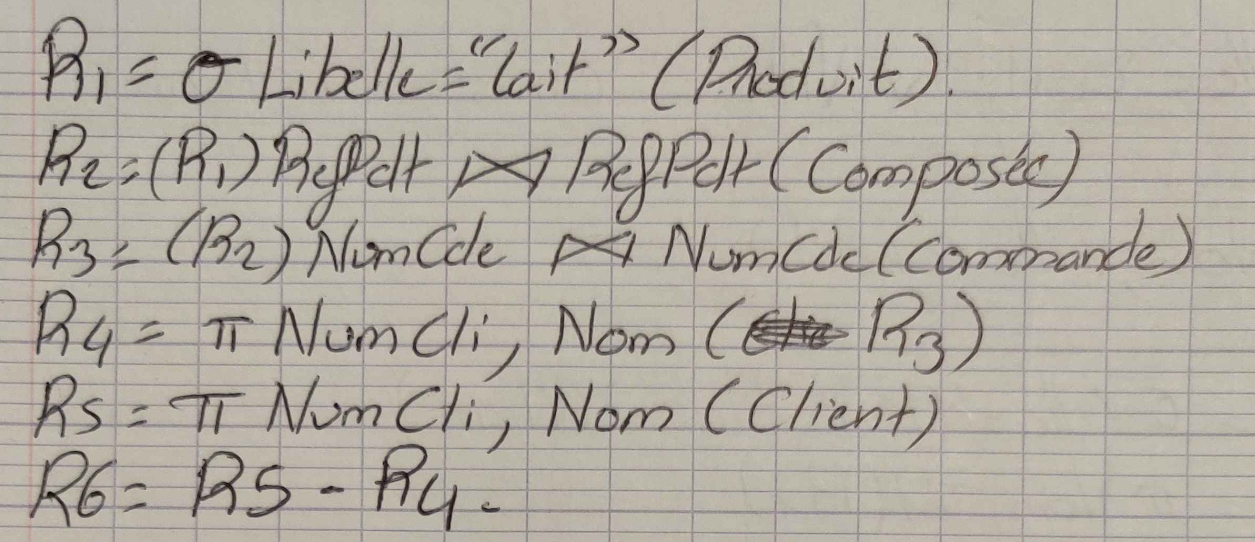
\includegraphics[width=0.7\textwidth]{alg/8.png}
  \label{fig:alg-rel}
\end{figure}

\begin{figure}[H]
  \centering
  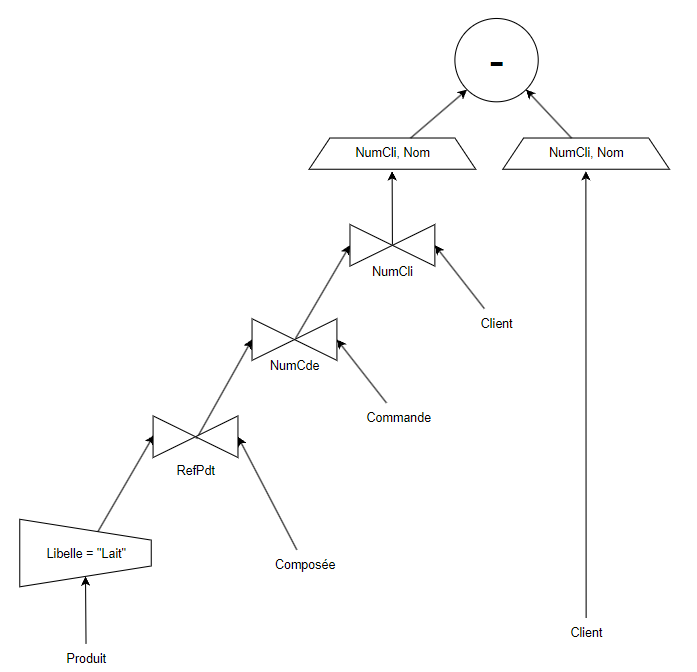
\includegraphics[width=0.5\textwidth]{algRel/8.png}
  \label{fig:alg-rel}
\end{figure}


\subsubsection{SQL}

\begin{lstlisting}[language=SQL]
  SELECT cl.NumCli, cl.Nom 
  FROM Client cl
  WHERE cl.NumCli NOT IN (
      SELECT cl.NumCli
      FROM Commande c
      JOIN Composee cp ON c.NumCde = cp.NumCde
      JOIN Produit p ON cp.RefPdt = p.RefPdt
      WHERE cl.NumCli = c.NumCli AND p.Libelle = 'lait'
  );
\end{lstlisting}

Version sans JOIN :

\begin{lstlisting}[language=SQL]
  SELECT cl.NumCli, cl.Nom 
  FROM Client cl
  WHERE cl.NumCli NOT IN (
      SELECT cl.NumCli
      FROM Commande c, Composee cp, Produit p
      WHERE c.NumCde = cp.NumCde 
        AND cp.RefPdt = p.RefPdt 
        AND cl.NumCli = c.NumCli 
        AND p.Libelle = 'lait'
  );
\end{lstlisting}

\subsection{Noms des clients ayant acheté des produits dont le prix est supérieur à 4 Euros}

\subsubsection{Algèbre Relationnelle}

\begin{figure}[H]
  \centering
  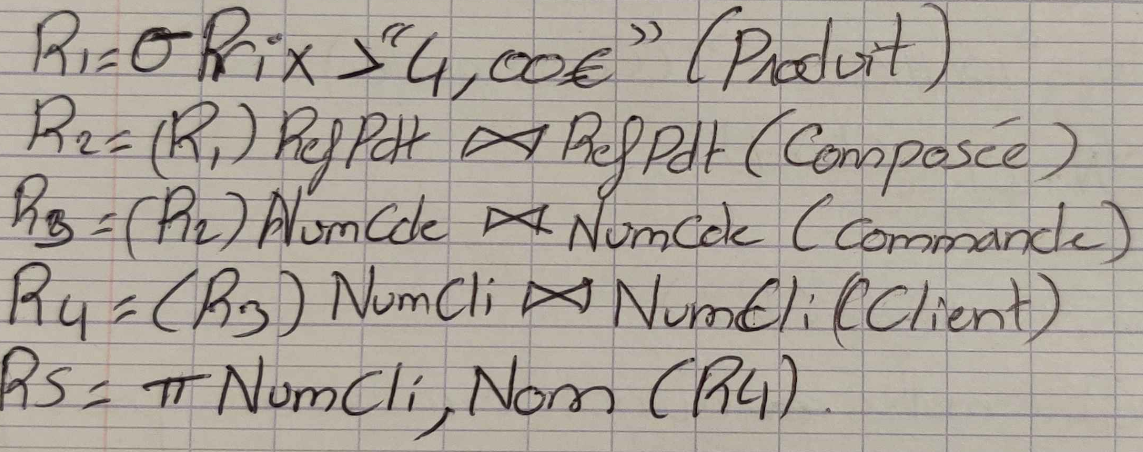
\includegraphics[width=0.7\textwidth]{alg/9.png}
  \label{fig:alg-rel}
\end{figure}

\begin{figure}[H]
  \centering
  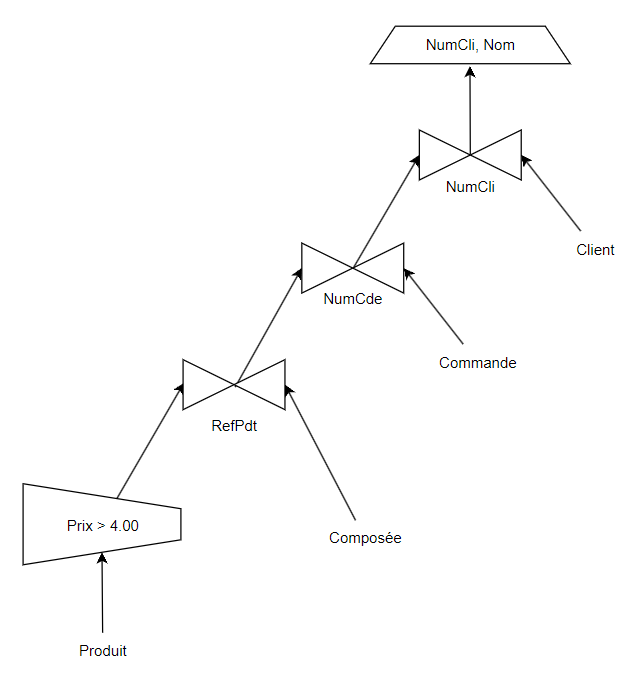
\includegraphics[width=0.5\textwidth]{algRel/9.png}
  \label{fig:alg-rel}
\end{figure}


\subsubsection{SQL}

\begin{lstlisting}[language=SQL]
  SELECT cl.NumCli cl.Nom 
  FROM Client cl
  JOIN Commande c ON cl.NumCli = c.NumCli
  JOIN Composee cp ON c.NumCde = cp.NumCde
  JOIN Produit p ON cp.RefPdt = p.RefPdt
  WHERE p.Prix > 4;
\end{lstlisting}

Version sans JOIN :

\begin{lstlisting}[language=SQL]
  SELECT cl.NumCli cl.Nom 
  FROM Client cl, Commande c, Composee cp, Produit p
  WHERE cl.NumCli = c.NumCli 
    AND c.NumCde = cp.NumCde 
    AND cp.RefPdt = p.RefPdt 
    AND p.Prix > 4;
\end{lstlisting}

\subsection{Liste des produits achetés par des porto-vecchiais}

\subsubsection{Algèbre Relationnelle}

\begin{figure}[H]
  \centering
  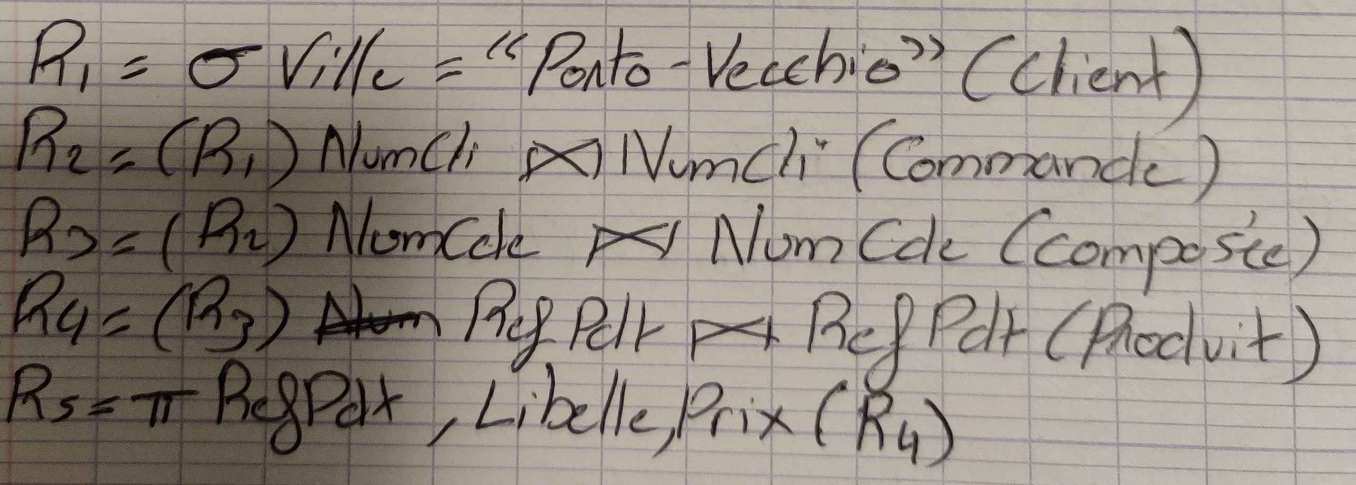
\includegraphics[width=0.7\textwidth]{alg/10.png}
  \label{fig:alg-rel}
\end{figure}

\begin{figure}[H]
  \centering
  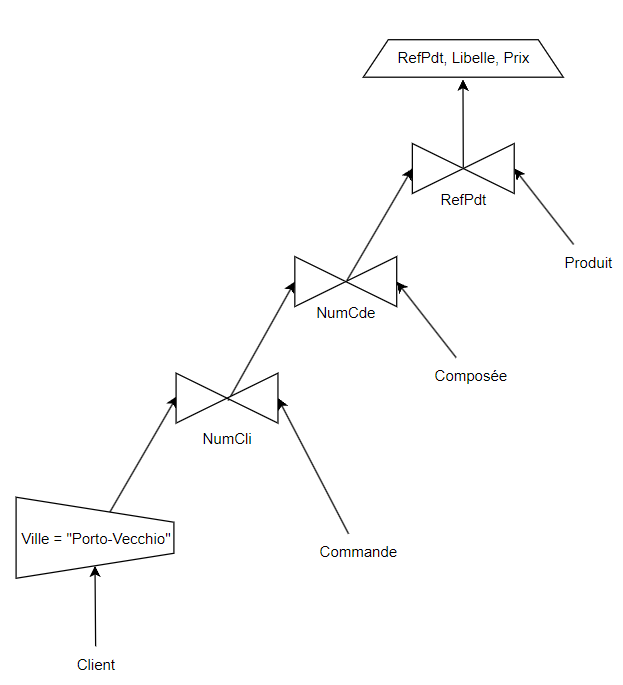
\includegraphics[width=0.5\textwidth]{algRel/10.png}
  \label{fig:alg-rel}
\end{figure}


\subsubsection{SQL}

\begin{lstlisting}[language=SQL]
  SELECT DISTINCT p.Libelle 
  FROM Produit p
  JOIN Composee cp ON p.RefPdt = cp.RefPdt
  JOIN Commande c ON cp.NumCde = c.NumCde
  JOIN Client cl ON c.NumCli = cl.NumCli
  WHERE cl.Ville = 'Porto-Vecchio';
\end{lstlisting}

Version sans JOIN :

\begin{lstlisting}[language=SQL]
  SELECT DISTINCT p.Libelle 
  FROM Produit p, Composee cp, Commande c, Client cl
  WHERE p.RefPdt = cp.RefPdt 
    AND cp.NumCde = c.NumCde 
    AND c.NumCli = cl.NumCli 
    AND cl.Ville = 'Porto-Vecchio';
\end{lstlisting}

\break\section{Question 3}

\subsection{Création de la base de données}

\begin{lstlisting}[language=SQL]
  CREATE TABLE Client (
      NumCli INT PRIMARY KEY, 
      Nom VARCHAR(50) NOT NULL, 
      Adresse VARCHAR(100), 
      CP CHAR(5), 
      Ville VARCHAR(50), 
      Tel VARCHAR(15)
  );
  
  CREATE TABLE Produit (
      RefPdt INT PRIMARY KEY, 
      Libelle VARCHAR(100) NOT NULL, 
      Prix DECIMAL(10, 2) NOT NULL
  );
  
  CREATE TABLE Commande (
      NumCde INT PRIMARY KEY, 
      Date DATE NOT NULL, 
      Montant DECIMAL(10, 2), 
      NumCli INT NOT NULL, 
      FOREIGN KEY (NumCli) REFERENCES Client(NumCli)
  );
  
  CREATE TABLE Composee (
      NumCde INT NOT NULL, 
      RefPdt INT NOT NULL, 
      Quantite INT NOT NULL, 
      PRIMARY KEY (NumCde, RefPdt), 
      FOREIGN KEY (NumCde) REFERENCES Commande(NumCde), 
      FOREIGN KEY (RefPdt) REFERENCES Produit(RefPdt)
  );
\end{lstlisting}

\subsection*{11. Total des commandes du client 102}

J'ai interprété cette question de deux manières différentes : le \textbf{montant total} des commandes du client 102 et le \textbf{nombre total} de commandes du client 102.

\subsubsection{Montant total des commandes du client 102}

\begin{lstlisting}[language=SQL]
  SELECT SUM(co.Montant) as "Montant total des commandes du client 102"
  FROM Commande co
  WHERE co.NumCli = 102;
\end{lstlisting}

\subsubsection{Nombre total de commandes du client 102}

\begin{lstlisting}[language=SQL]
  SELECT COUNT(co.NumCde) as "Nombre total de commandes du client 102"
  FROM Commande co
  WHERE co.NumCli = 102;
\end{lstlisting}

\subsection*{12. Montant moyen des commandes}

\begin{lstlisting}[language=SQL]
  SELECT AVG(co.Montant) as "Montant moyen des commandes"
  FROM Commande co;
\end{lstlisting}

\subsection*{13. Nombre des clients}

\begin{lstlisting}[language=SQL]
  SELECT COUNT(cl.NumCli) as "Nombre des clients"
  FROM Client cl;
\end{lstlisting}

\end{document}